%Beamer class
\documentclass{beamer}

\usepackage[czech]{babel}
\usepackage[utf8]{inputenc}
\usepackage{fontenc}
\usepackage{tgheros}
\usepackage{array}
\usepackage{color}
\usepackage{hyperref}


\usetheme{AnnArbor}
\usecolortheme{crane}


\title[B0B13KEO]{B0B13KEO}
\subtitle[KEO] {Konstrukce a realizace elektronických obvodů}
\author[Brejcha]{\texorpdfstring{Michal Brejcha\newline\url{brejcmic@fel.cvut.cz}}{Michal Brejcha}}
\institute[ČVUT]{ČVUT v Praze, FEL}
\date[Praha, 2022]{Praha, 2022}

%------------------------------------------------------------------------------
%Konstanty a definice
%------------------------------------------------------------------------------
\newtheorem{myDef}{}

\begin{document}
%------------------------------------------------------------------------------
%Uvodni slajd
%------------------------------------------------------------------------------
\frame{\titlepage}

\begin{frame}
\frametitle{Obsah} 
\tableofcontents
\end{frame}

\AtBeginSection[]
{
  \begin{frame}
    \frametitle{Téma}
    \tableofcontents[currentsection]
  \end{frame}
}

%------------------------------------------------------------------------------
%Bezpecnost
%------------------------------------------------------------------------------
\section{\texorpdfstring{Bezpečnost}{Bezpecnost}}
%------------------------------------------------------------------------------
	\begin{frame}
    \frametitle{Základní pravidla bezpečnosti}
		\begin{itemize}
		\item Vstup do laboratoří a práce v laboratoři jsou dovoleny jen za přítomnosti učitele.
		\item Manipulace s přístrojovým vybavením laboratoře je dovolena jen v prostorách laboratoře.
		\item Zapínání laboratorních stolů (případně jiných zařízení nn) je dovoleno jen se souhlasem a dohledem učitele.
		\item \textbf{\color{red}{Laboratorní stůl nebo celou laboratoř je dovoleno (jste povinni) kdykoliv vypnout bez výstrahy v případě hrozícího nebezpečí. \uv{BEZPEČNOSTNÍ TLAČÍTKA}}}
		\end{itemize}
	\end{frame}
%------------------------------------------------------------------------------
	\begin{frame}
    \frametitle{Omezení a předpisy}
		\begin{itemize}
		\item V laboratoři není dovolena konzumace potravin,
    \item z laboratoře není dovoleno odnášet jakékoliv přístroje a vlastní přístroje je možné použít (připojit na napájení, měřit s nimi apod.) jen po dohodě s učitelem,
		\item není dovoleno používání mobilních telefonů v průběhu výuky uvnitř laboratoře, pokud se nejedná o případ tísňového volání,
		\item studenti jsou povinni dodržovat zásady protipožární ochrany,
		\item závady na zařízení je nutné ihned hlásit vyučujícímu.
		\end{itemize}
	\end{frame}
%------------------------------------------------------------------------------
	\begin{frame}
    \frametitle{Rizika}
		\begin{itemize}
		\item Úraz elektrickým proudem: práce s nn, přítomnost nekrytých svorek na laboratorním stole.
		\item Popáleniny: páječka - pájení, chybný návrh - horká součástka.
		\item Řezné nebo tržné rány: odizolování vodičů pomocí nože, rozšiřování vrtaných otvorů.
		\item Otrava nebo poleptání chemikáliemi: použití rozpouštědel při mytí pcb, použití chemie při pájení.
		\end{itemize}
	\end{frame}
%------------------------------------------------------------------------------
	\begin{frame}
    \frametitle{Univerzální postup v případě nebezpečí}
		\begin{enumerate}
		\item Zajištění bezpečnosti:\\
		rozpojení elektrického obvodu (bezpečnostní tlačítka), odpojení přítomných přístrojů, uzavření příp. odstranění nebo zabránění šíření (louže - těkavé látky) chemických látek
		\item První pomoc postiženému:\\ chlazení popáleného místa studenou vodou, zastavení krvácení, umělé dýchání, nepřímá srdeční masáž.
		\item Upozornění lektora (zodpovědného pracovníka laboratoří), na vzniklou situaci.
		\item Přivolání lékařské pomoci (tel.: 155), uvědomění vrátnice (tel.: 2222).
		\end{enumerate}
	\end{frame}
%------------------------------------------------------------------------------
	\begin{frame}
    \frametitle{Požární bezpečnost - povinnosti}
		\begin{enumerate}
		\item Počínat si tak, aby nedocházelo ke vzniku požáru, zejména při používání tepelných, elektrických, plynových a jiných spotřebičů, při skladování a používání hořlavých nebo požárně nebezpečných látek, manipulaci s nimi nebo otevřeným ohněm či jiným zdrojem zapálení
		\item Neomezovat přístup k rozvodným zařízením elektrické energie a k uzávěrům vody a topení.
		\end{enumerate}
	\end{frame}
%------------------------------------------------------------------------------
	\begin{frame}
    \frametitle{Požární bezpečnost - zdolávání požáru}
		\begin{enumerate}
		\item Hlasitým opakovaným voláním (\textbf{HOŘÍ!}) vyhlásit požární poplach pro své okolí.
		\item Provést nutná opatření pro záchranu ohrožených osob.
    \item Uhasit požár, je\-li to možné, nebo provést nutná opatření k zamezení jeho šíření.
    \item Ohlásit neodkladně na určeném místě zjištěný požár ev. zabezpečit jeho ohlášení (tel.: 150).
    \item Ostatní osoby opustí spořádaně budovu a soustředí se na shromaždišti. V době požárního poplachu je přísně \textbf{zakázáno používat výtah!}
		\end{enumerate}
	\end{frame}
%------------------------------------------------------------------------------
%Napln cviceni
%------------------------------------------------------------------------------
\section{\texorpdfstring{Náplň cvičení}{Napln Cviceni}}
%------------------------------------------------------------------------------
  \begin{frame}
    \frametitle{Osnova cvičení}
		\begin{enumerate}
          \small
          \item Úvod. Bezpečnostní předpisy. Zadání témat.
          \item Praktické provedení elektronického obvodu. Ukázky prací studentů z jiných let.
          \item Prezentace elektronických obvodů zamýšlených k výrobě.
          \item Návrh DPS programem KiCAD.
          \item Návrh DPS programem KiCAD.
          \item Ověření funkce určité části obvodu v laboratoři.
          \item Kontrola návrhů, podkladů a generování výrobních dat pro výrobu (\textbf{nutný hotový návrh})
          \item Specifické vlastnosti elektronických součástek
          \item Vrtání DPS, kontrola DPS, úpravy DPS do krabiček
          \item Realizace elektronického obvodu – pájení 
          \item Uvádění elektronického obvodu do provozu
          \item Ověřování funkce obvodu a měření
          \item Závěrečná zpráva
          \item Zápočet
		\end{enumerate}
	
	\end{frame}
%------------------------------------------------------------------------------
	\begin{frame}
    \frametitle{Zápočet}
		
		\begin{itemize}
			\item Předvést funkci výrobku,
			\item odevzdat zprávu o výrobku:
      
      \begin{itemize}
        \item Název výrobku, jméno studenta, datum.
        \item Úplné zadání (funkce, parametry, rozsahy apod.).
        \item Popis funkce, výpočty obvodů, schéma zapojení.
        \item Otisk DPS, osazovací schéma.
        \item Rozpiska součástek.
        \item Výsledky měření.
        \item Zhodnocení.
      \end{itemize}
		\end{itemize}
	
	\end{frame}
%------------------------------------------------------------------------------
	\begin{frame}
    \frametitle{Výroba elektronického obvodu}
		
		\begin{itemize}
			\item DPS vyrábí a platí škola,
			\item součástky kupuje student.
			\item Návrh obvodu lze získat od jiného autora - např. knížka, web...
			\item Pokud již existuje dps, lze ji použít pro inspiraci, nicméně předpokládají se vlastní úpravy řešitele a hlavně její překreslení v návrhovém programu.
		\end{itemize}
	
	\end{frame}
%------------------------------------------------------------------------------
	\begin{frame}
    \frametitle{Vlastnosti zadání}
		
		\begin{itemize}
			\item Obvod s minimálně 30 součástkami,
			\item převážně THT montáž (jednovrstvý plošný spoj nebo dvouvrstvý \textbf{bez prokovů}),
      \item napájení výhradně malým napětím,
      \item vyhýbejte se programovatelným součástkám,
      \item pokud chcete procesor, tak Arduino (snadné ověření funkce obvodu),
      \item jen nízkofrekvenční obvody, 
      \item na relativně malé výkony.
		\end{itemize}
	
	\end{frame}
%------------------------------------------------------------------------------
	\begin{frame}
    \frametitle{Příklad jednoduchého obvodu $>$30 součástek}
		\textbf{Voltmetr Arduino}
		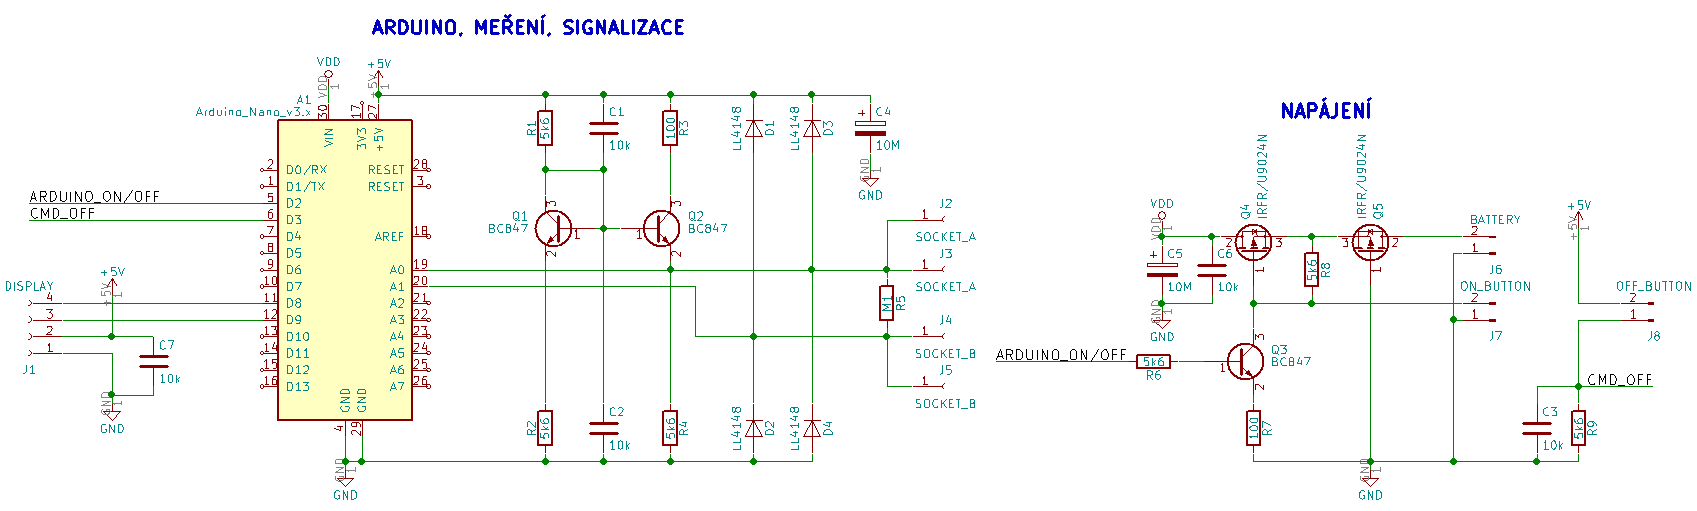
\includegraphics[scale=0.24]{obr/eo_voltSch.png}
	
	\end{frame}
%------------------------------------------------------------------------------
	\begin{frame}
    \frametitle{Příklad jednoduchého obvodu $>$30 součástek}
		\textbf{Měření charakteristické impedance kabelu}
    \begin{center}
      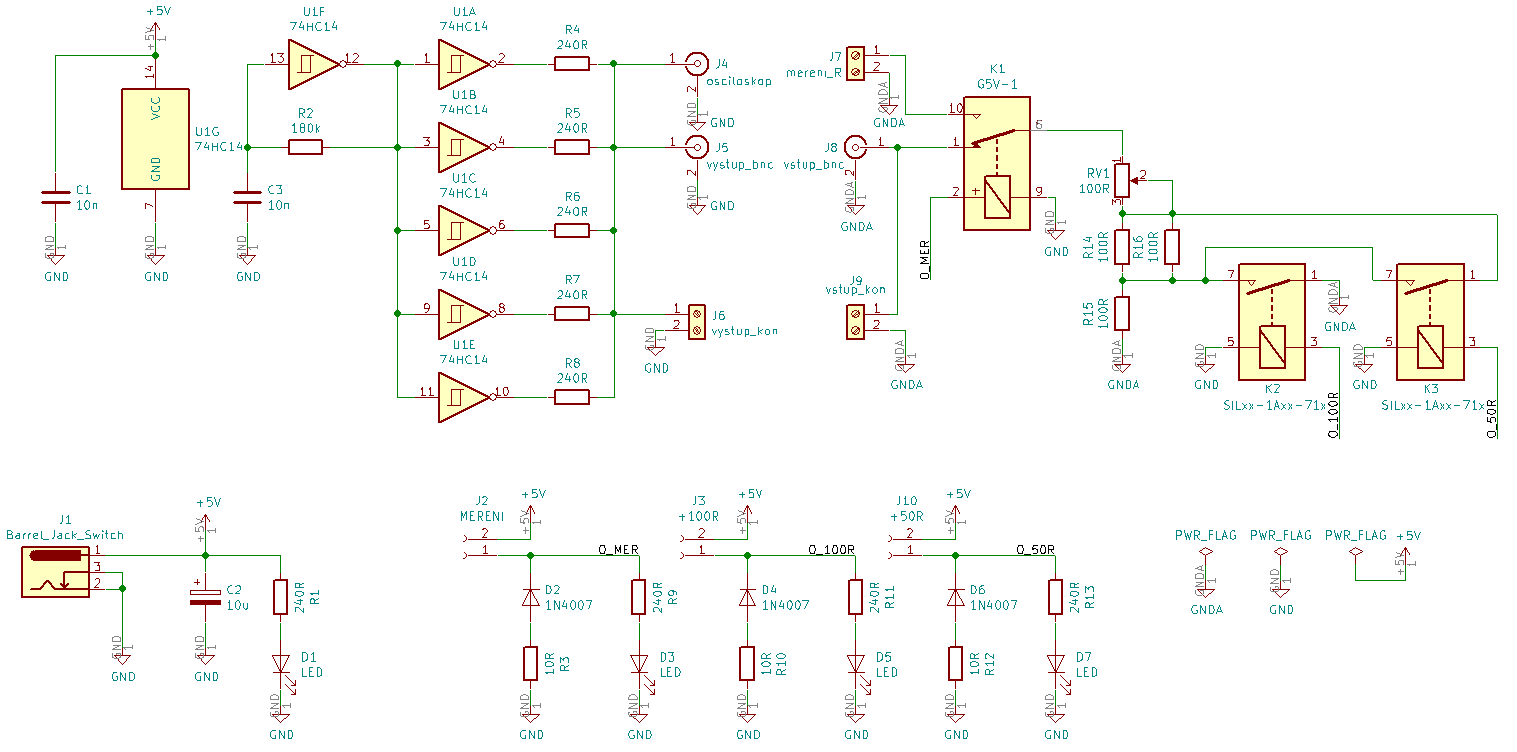
\includegraphics[scale=0.26]{obr/eo_impSch.png}
    \end{center}
	
	\end{frame}
%------------------------------------------------------------------------------
	\begin{frame}
    \frametitle{Příklad jednoduchého obvodu $>$30 součástek}
		\textbf{Signalizace ztráty napájení}
    \begin{center}
      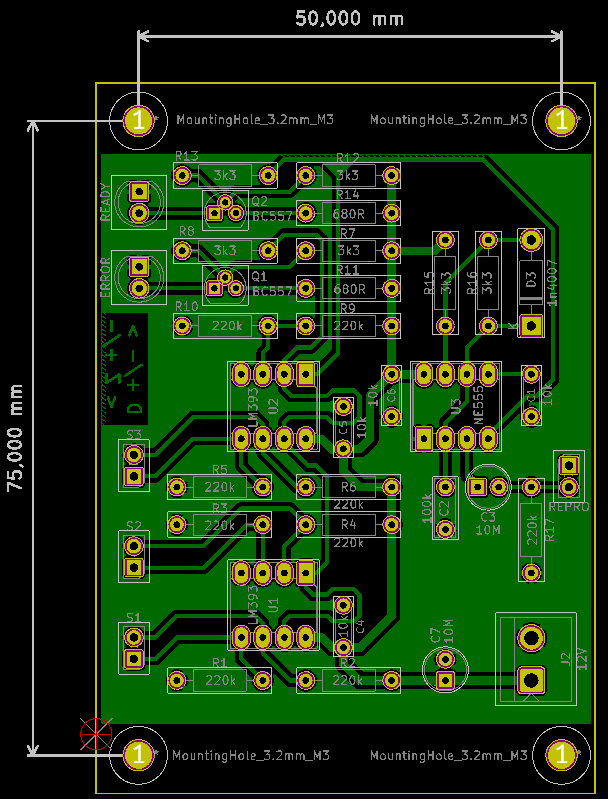
\includegraphics[scale=0.26]{obr/eo_detBrd.png}
    \end{center}
	
	\end{frame}
%------------------------------------------------------------------------------
	\begin{frame}
    \frametitle{Co potřebuji na příští hodinu?}
    
    \begin{enumerate}
      \item Schéma zapojení obvodu, který chci vytvořit (na papíře).
      \item Seznam parametrů obvodu, např.: napájecí napětí, vstupní a výstupní
      impedance, typ zátěže, generované frekvence, atd.
      \item Seznam součástek - GME.
    \end{enumerate}
    
    
    \textbf{Poznámka:} \\
    Minimálně je potřeba mít schéma zapojení obvodu, zbytek můžeme vypracovat na hodině.
	
	\end{frame}
%------------------------------------------------------------------------------
%Prezentace studentskych praci
%------------------------------------------------------------------------------
\section{\texorpdfstring{Prezentace studentských prací}{Prezentace studentskych praci}}
%------------------------------------------------------------------------------
\begin{frame}
    \frametitle{Požadavky na prezentaci}
		
    \textbf{Stačí 3 stránky v Powerpointu.}
    \begin{enumerate}
      \item Seznámení s projektem = co chci dělat?
      \item Cílové parametry obvodu = čeho chci dosáhnout?
			
			\begin{itemize}
				\item pro zdroje například výstupní napětí, proudy, výkon,
				\item pro zesilovače například zesílení, zkreslení, výkon,
				\item pro logický obvod například co má řídit a jak, ...
			\end{itemize}
			
			\item Ukázka toho, z čeho obvod bude vycházet = co je mým zdrojem informací?
			
    \end{enumerate}
		
		\textbf{Prezentace se nakonec odevzdává do moodle.}
	
	\end{frame}
%------------------------------------------------------------------------------
	\begin{frame}
    \frametitle{Ukázka prezentace - David Puchoň}
		
		
\includegraphics[page=1,width=0.9\textwidth]{pdf/KEO-David_Puchon-Prezentace.pdf}
	
	\end{frame}
%------------------------------------------------------------------------------
	\begin{frame}
    \frametitle{Ukázka prezentace - David Puchoň}
		
		
\includegraphics[page=2,width=0.9\textwidth]{pdf/KEO-David_Puchon-Prezentace.pdf}
	
	\end{frame}
%------------------------------------------------------------------------------
	\begin{frame}
    \frametitle{Ukázka prezentace - David Puchoň}
		
		
\includegraphics[page=3,width=0.9\textwidth]{pdf/KEO-David_Puchon-Prezentace.pdf}
	
	\end{frame}
%------------------------------------------------------------------------------
	\begin{frame}
    \frametitle{Ukázka prezentace - David Puchoň}
		
		
\includegraphics[page=4,width=0.9\textwidth]{pdf/KEO-David_Puchon-Prezentace.pdf}
	
	\end{frame}
%------------------------------------------------------------------------------
%Prezentace studentskych praci
%------------------------------------------------------------------------------
\section{\texorpdfstring{Ukázka závěrečné práce}{Ukazka zaverecne prace}}
%------------------------------------------------------------------------------
	\begin{frame}
    \frametitle{Obsah závěrečné práce}
		
		\begin{itemize}
			\item Název výrobku, jméno studenta, datum.
			\item Úplné zadání (funkce, parametry, rozsahy apod.).
			\item Popis funkce, výpočty obvodů, schéma zapojení.
			\item Otisk DPS, osazovací schéma.
			\item Rozpiska součástek.
			\item Výsledky měření.
			\item Zhodnocení.
		\end{itemize}
	
	\end{frame}
%------------------------------------------------------------------------------
	\begin{frame}
    \frametitle{Závěrečná práce Petr David}
		
		\begin{columns}
			\begin{column}{0.5\textwidth}
				 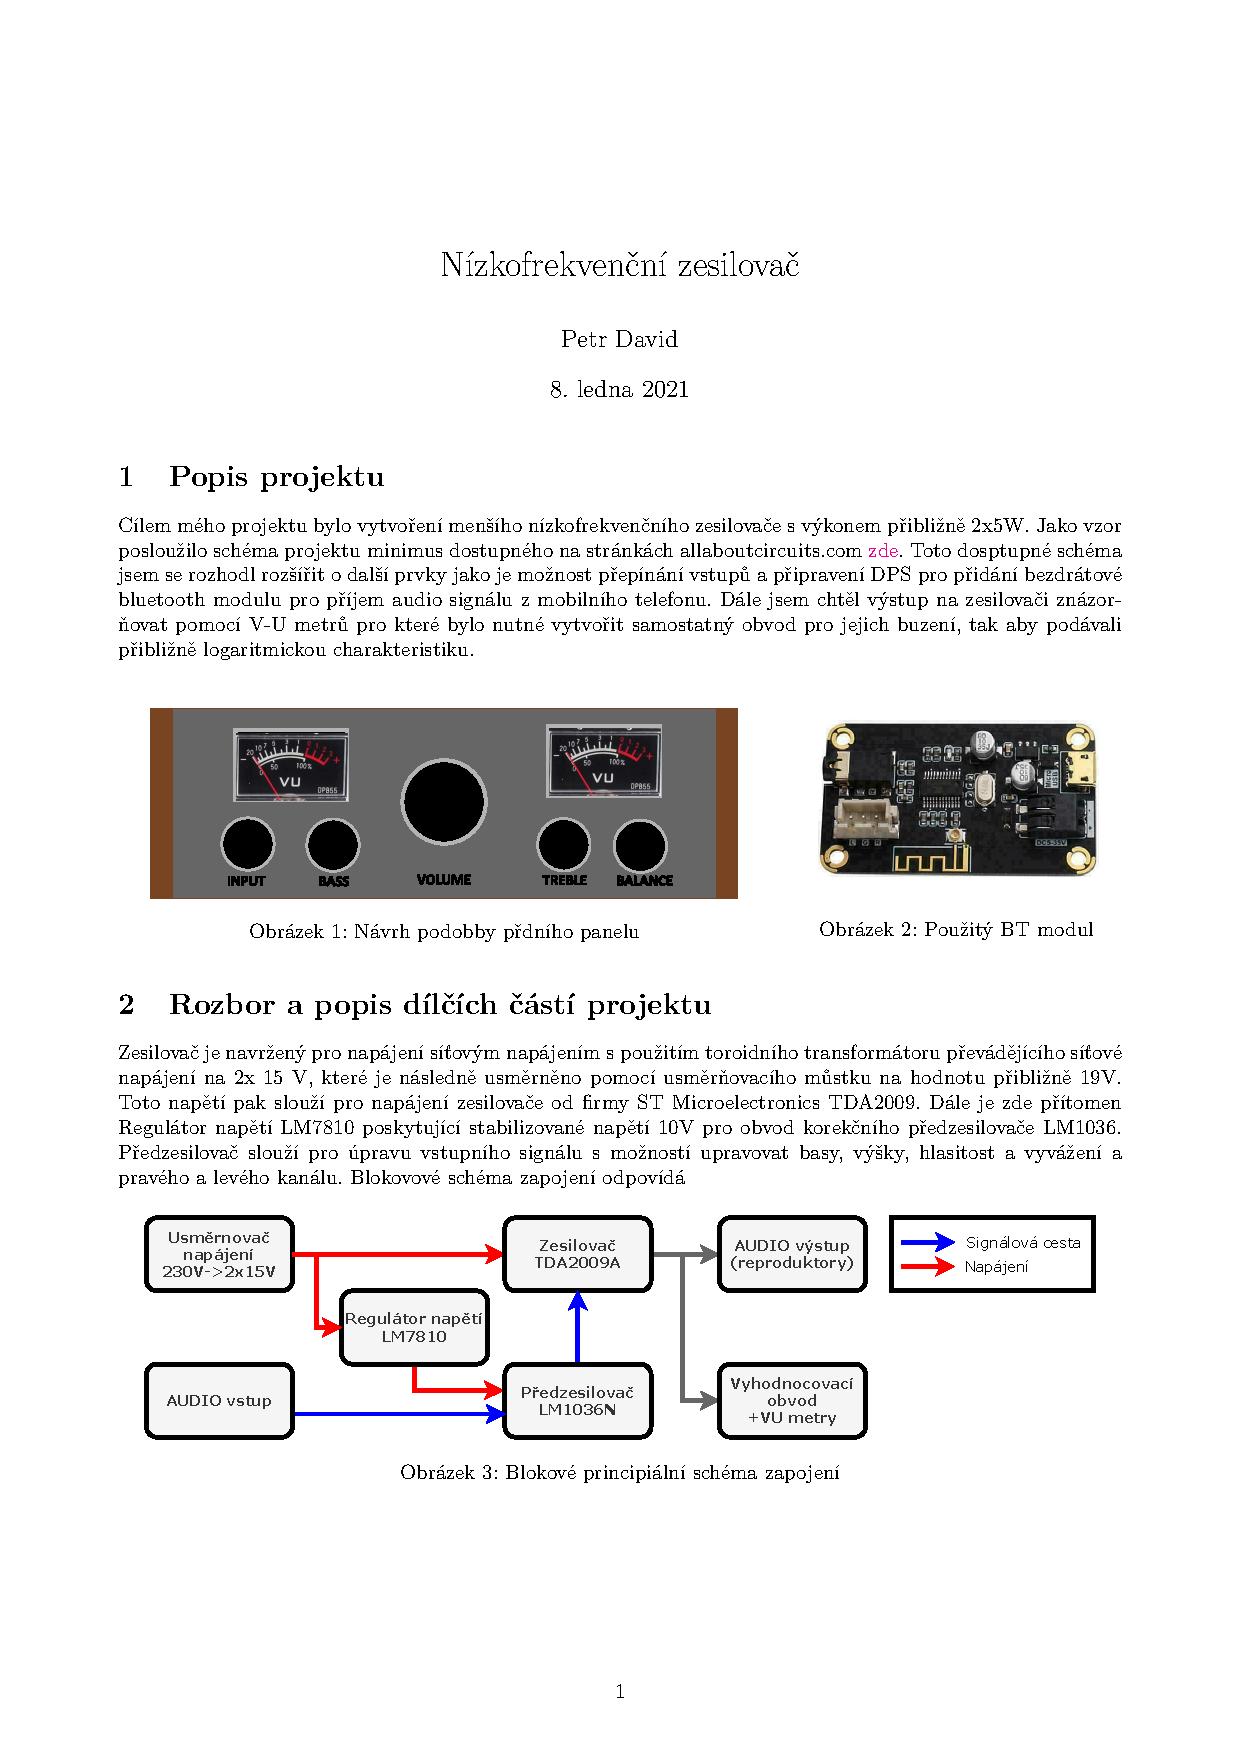
\includegraphics[page=1,width=5cm]{pdf/KEO-Petr_David-ZP.pdf}
			\end{column}
			\begin{column}{0.5\textwidth} 
				 \includegraphics[page=2,width=5cm]{pdf/KEO-Petr_David-ZP.pdf}
			\end{column}
		\end{columns}
	
	\end{frame}
%------------------------------------------------------------------------------
	\begin{frame}
    \frametitle{Závěrečná práce Petr David}
		
		\begin{columns}
			\begin{column}{0.5\textwidth}
				 \includegraphics[page=3,width=5cm]{pdf/KEO-Petr_David-ZP.pdf}
			\end{column}
			\begin{column}{0.5\textwidth} 
				 \includegraphics[page=4,width=5cm]{pdf/KEO-Petr_David-ZP.pdf}
			\end{column}
		\end{columns}
	
	\end{frame}
%------------------------------------------------------------------------------
	\begin{frame}
    \frametitle{Závěrečná práce Iveta Kropáčková}
		
		\begin{columns}
			\begin{column}{0.5\textwidth}
				 \includegraphics[page=1,width=5cm]{pdf/KEO-Iveta_Kropackova-ZP.pdf}
			\end{column}
			\begin{column}{0.5\textwidth} 
				 \includegraphics[page=2,width=5cm]{pdf/KEO-Iveta_Kropackova-ZP.pdf}
			\end{column}
		\end{columns}
	
	\end{frame}
%------------------------------------------------------------------------------
	\begin{frame}
    \frametitle{Závěrečná práce Iveta Kropáčková}
		
		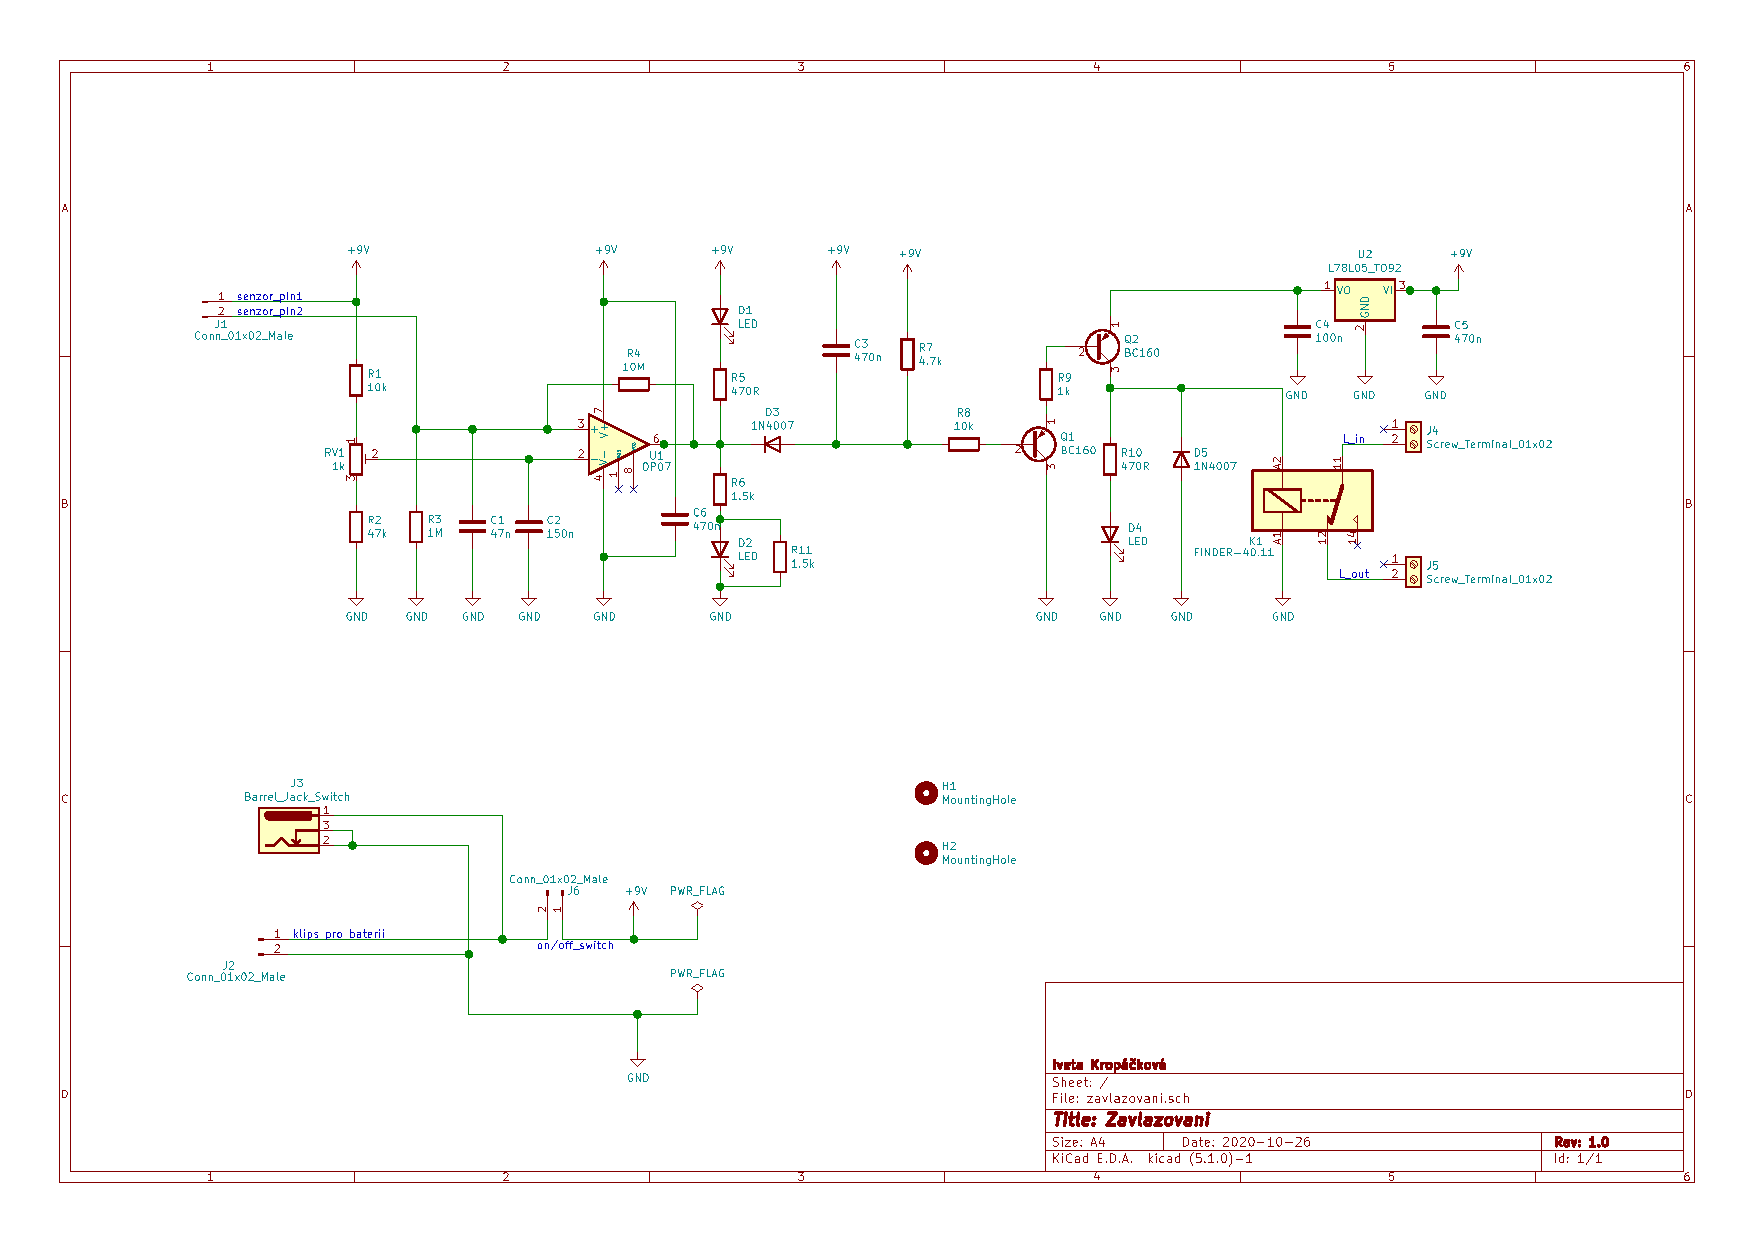
\includegraphics[page=1,width=0.95\textwidth]{pdf/KEO-Iveta_Kropackova-schema.pdf}
	
	\end{frame}
%------------------------------------------------------------------------------
	\begin{frame}
    \frametitle{Závěrečná práce Iveta Kropáčková}
		
		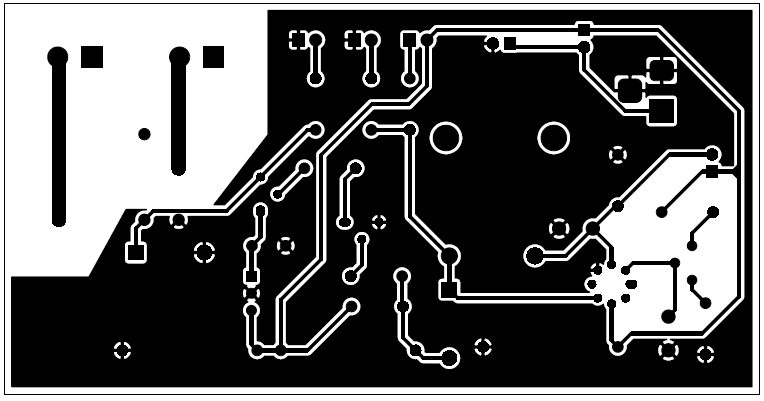
\includegraphics[width=0.95\textwidth]{obr/kropackova-pcb.png}
	
	\end{frame}
%------------------------------------------------------------------------------
	\begin{frame}
    \frametitle{Závěrečná práce Iveta Kropáčková}
		
		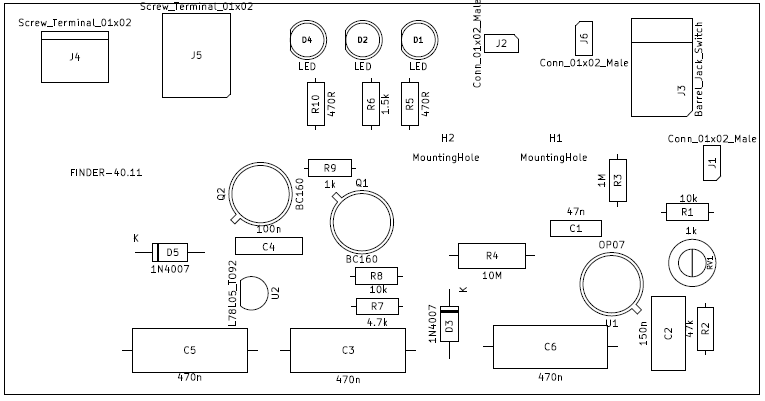
\includegraphics[width=0.95\textwidth]{obr/kropackova-osaz}
	
	\end{frame}
%------------------------------------------------------------------------------
	\begin{frame}
    \frametitle{To je vše...}
		
		\begin{center}
			\textbf{Děkuji za pozornost}
		\end{center}
	
	\end{frame}
%------------------------------------------------------------------------------

\end{document}